\documentclass[man]{apa2}
\usepackage{pslatex}
\usepackage{amssymb}
\usepackage{graphicx}
\usepackage{color}
\usepackage{covington}
\usepackage[usenames,dvipsnames]{xcolor}
\usepackage{booktabs}
\usepackage{setspace}


\title{Understanding the effect of social context on learning: \\ A replication of Xu and Tenenbaum (2007b)}

\twoauthors{Molly L. Lewis}{Michael C. Frank}
\twoaffiliations{Department of Psychology, Stanford University}{Department of Psychology, Stanford University}


\abstract{

~\\

Keywords: word learning, induction, Bayesian inference}

\shorttitle{Replication of Xu and Tenenbaum 2007b}
\rightheader{Replication of Xu and Tenenbaum 2007b}

\acknowledgements{ 

~\\

\noindent Address all correspondence to Molly L. Lewis, Stanford University, Department of Psychology, Jordan Hall, 450 Serra Mall (Bldg. 420), Stanford, CA, 94305. Phone: 650-721-9270. E-mail: \texttt{mll@stanford.edu}}

\begin{document}

\maketitle              


\section{Introduction}
Imagine you were on a hike and saw a rock positioned oddly at an ambiguous intersection of trails.  If you thought you were on a trail  which no one had traveled in years, you probably wouldn't think much of that rock. But, if you knew your  campmate had traveled that same trail earlier that day, you might interpret the rock differently: You might interpret the rock as a sign intended to point you to the correct path. This intuition---that the  source of a piece of information influences the strength of the inference to be drawn---suggests that social information may have a privileged role in human learning.

\citeA{xu2007} examine this phenomenon in the context of a particularly difficult inductive problem: Concept generalization in word learning. Faced with a novel word and its referent, children must decide between an infinite number of hypotheses about the concept extension of that word. For example, consider a child who hears the word  ``banana" in the context of a single banana on a table. While the referent of that object is clear in the moment of language use (i.e., the particular banana on the table), the broader concept is highly ambiguous: ``banana" could refer to the category of bananas, the category of fruit, that particular species of banana (e.g., plantains), yellow things, or any number of other ad-hoc categories. 

\citeA{xu2007} ask whether children make use of the information source about a new word to guide their inferences about how to generalize its meaning. In particular, they test a prediction that falls out of their word learning model. In their Bayesian model, learners observe data as word-object pairs and make inferences about the concept associated with that word from a hypothesis space of all possible meanings. Critically, the model predicts that  an ideal  learner should generalize more broadly when the exemplar is sampled from the full hypothesis space of meanings ({\it weak sampling}), and should generalize more narrowly when the exemplar is sampled from only  the true concept of the word within the full hypothesis space ({\it strong sampling}). 

In their experiment, \citeA{xu2007} manipulate  sampling  ``strength"  through  the presentation source of the data: The learner is either presented with three exemplars of the target word from a knowledgeable teacher or the learner makes (correct) guesses about the referent of the word. Since the teacher  knows the true concept, the data are sampled strongly from only the true concept. But, in the learner-generated condition, the learner is naive about the true underlying concept and thus the data are sampled weakly from the full hypothesis space.  The key prediction is that, given a hypothesis space with hierarchical concepts (basic, subordinate, superordinate; i.e.,  banana, plantain, fruit),  participants in the teacher condition should be more likely to generalize broadly to the basic level, while participants in the learner condition should generalize conservatively to only the subordinate condition. Their data strongly support this prediction in both adults ($d = 1.74\ [.47,\ 3.01]$) and children  ($d = .98\ [.29,\ 1.67]$).


There are a number of reasons to conduct a replication of this study. First, replication attempts of other predictions of this model have challenged this framework. This paper 
\cite{xu2007a}
\cite{spencer2011}
\cite{jenkins2015non}


There are additional reasons to conduct a replication of this particular study. \cite{navarro2012sampling}. More generally, evidence suggests that effects that rely on social manipulations are less likely to replicate than effects in more ``cognitive" domains \cite{reproProj2015}.

Finally, this study is important to replicate because the broad theoretical question---how the source of information influences learning---has far-reaching implications for our understanding of human learning. Every piece of data observed in the world, including the experimental context,  is observed in some social context. While the degree of this social pressure may vary (consider yourself observing flowers  alone in a forest versus a case observing flowers received from your partner on Valentine's day), humans are always part of a social system. Thus, in our effort to understand how learners make inferences on the basis of observations in the world, it is important to understand what factors influence this inference, and the source of these observations is likely an important factor.

The social context of human learning also has practical consequences for the interpretation of data collected in psychological experiments. This is because experimental data are often consistent with at least two accounts---an account that relies on  reasoning about the intention of the experimenter, and an account that relies on context-independent reasoning. Consider two examples. A well-known phenomenon in word learning is that children are biased to select a novel object for a novel word, given the presence of both a familiar and novel object \cite<often referred to as {\it mutual exclusivity} in the literature, >{markman1988}. This pattern is difficult to account for psychologically, however, because there are at least two accounts of this behavior. On the one hand, this result could be due to a context-independent bias to assume that lexicons are structured with one word mapping to one concept, and one concept mapping to one word. Another possibility relies on reasoning about the intentions of the experimenter (Why would the experimenter use a strange word to refer to the familiar object if she meant the familiar one? \cite{clark1987principle, clark1988logic})Both of these accounts make similar predictions, and are therefore difficult to disentangle empirically.

Another example of this interpretative ambiguity is the \citeA{heider1944} study. In their task, participants viewed a short movie showing several geometric shapes moving in a way that appeared to be contingent. Nearly all participants spontaneously interpreted the video as depicting animate  beings, rather than as simple shapes moving around. Like in the case of mutual exclusivity, there are at least two ways to interpret this result. One possibility is that participants rely on low level features of the scene to infer animacy (e.g., contingency), but another possibility is that participants infer the intention of the experimenter who created the videos and assume an animate intention. 

These two cases---mutual exclusivity and animacy projection---represent a sample of a pervasive theoretical issue in experimental psychology: Data consistent with both pragmatically rich  and  context-independent accounts.  There is not a simple solution to this empirical challenge because it is impossible to fully eliminate a social context from experimental paradigms. Our best bet, therefore, is to try to understand the influence of the social context on learning, and  \citeA{xu2007} represents a insightful attempt to systematically shed light on this practical issue.
%, in which participants projected animate qualities onto objectively inanimate stimuli. 

Thus, given the uncertainty associated with  the \citeA{xu2007} result, as well as its theoretical and practical significance, we sought to replicate it.  We conducted four replications of \citeA{xu2007}, three online and one in-lab.  Our data replicate the original effect, but suggest an effect much smaller in magnitude than the original report. In the General Discussion, we suggest a number of factors that may influence the magnitude of this effect that should be explored in future work.

%Given the relevance of this broader question, therefore, this study explores a domain that is particularly important to gain theoretical clarity. 

%All experimental data---and simply data more generally---is collected in a social context. 
%Difficult to interpret -- Hieder, ME -- because the inferences that are drawn are consistent with both a pragmatic inference as well as a context-independent inference. It is therefore important --- both for our understanding of how to interpret experimental results, as well as for our understanding of human learning more generally --- to understand how the source of information about the world influences learning.  The target study provides a key contribution to this question by directly manipulating the source of learners' data and asking how that influences learning.


%Both of the scenarios described above illustrate a property of human communicative behavior: Any act of communication is supported both by our context-dependent, pragmatic abilities and communicative biases encoded in the structure of language. To understand the psychological basis of these behaviors, we must disentangle these supports empirically. In this paper, we explore the nature of this empirical challenge, the evidence for its existence in each of the case studies we described, and a potential way forward.

\begin{figure}[t]
 \begin{center} 
  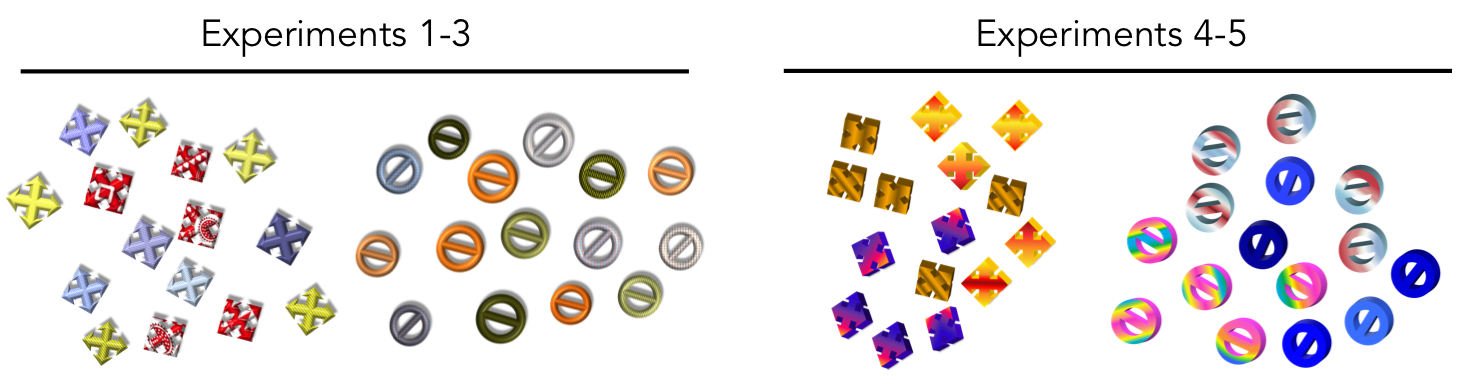
\includegraphics[width=5.8in]{figures/stims.png} 
  \caption{ \label{fig:stims} Sample stimuli used in Experiments 1-3 (left) and Experiment 4 (right). The Experiment 4 stimuli are intended to be maximally similar to the original Xu and Tenenbaum (2007b) stimuli, with lower subordinate-level variability than the stimuli used in Experiments 1-3. The full set of stimuli can be accessed here: xx. 
 } 
 \end{center} 
\end{figure}	

 \begin{figure} [t]
 \begin{center} 
  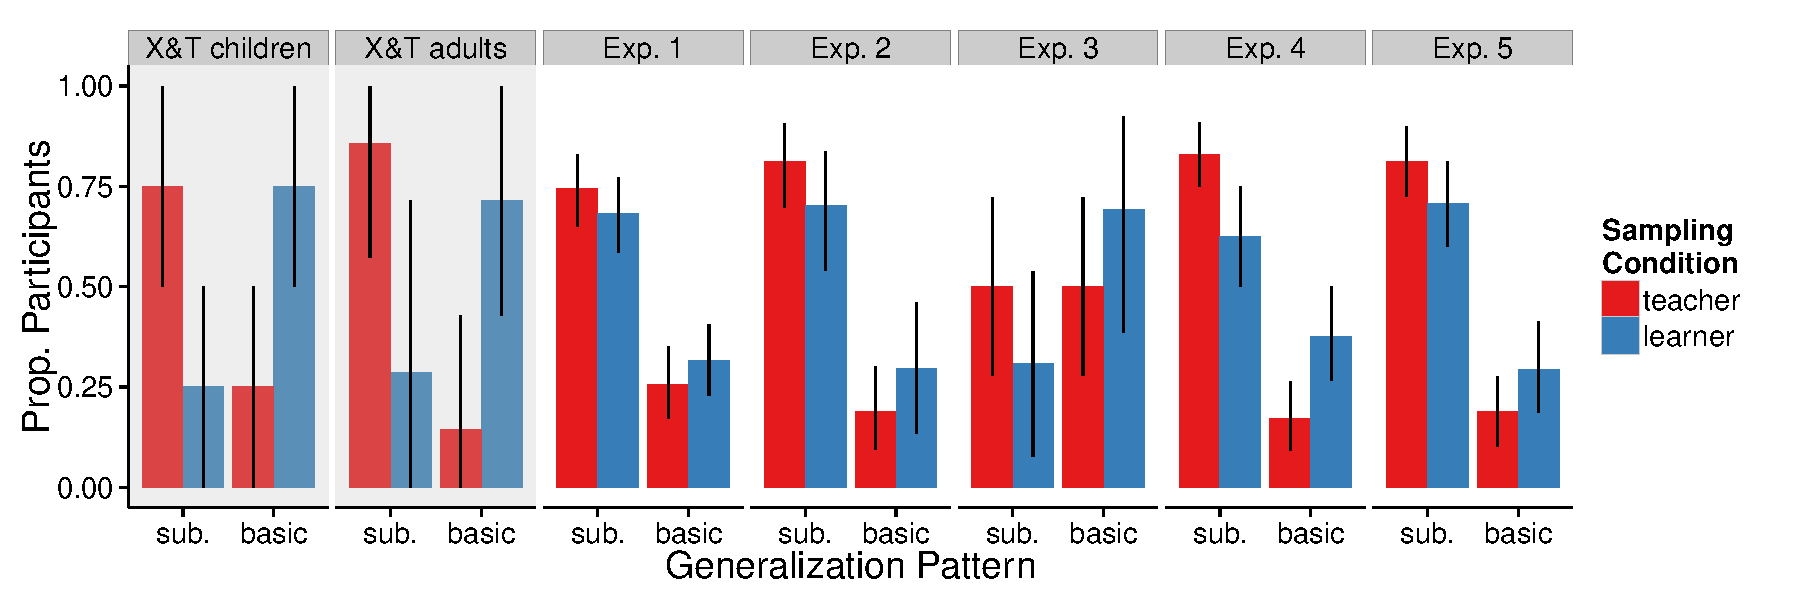
\includegraphics[width=6.5in]{figures/FIG_2.pdf} 
  \caption{\label{fig:bar_plots} Proportion participants generalizing to the subordinate (sub.) or basic level category in the original adult experiment ($N = 14$) and in our four replication attempts ($N_{1} = 14$; $N_{2} = 14$; $N_{3}  = 14$; $N_{4}  = 14$).  Experiments 1, 2, and 4 were conducted online, and Experiment 3 was conducted in-person. Proportions shown here are determined based on liberal criteria, described in the Main Text. Error bars reflect 95\% confidence intervals, calculated via non-parametric bootstrapping. } 
 \end{center} 
\end{figure}

  
\section{Experiment 1}

\subsection{Methods}

\subsubsection{Participants} 
\subsubsection{Stimuli}
\footnote{All stimuli, experiments, raw data and analysis code can be found at \url{XX}. 
Analyses can be found at: \url{XX}.} 


\subsubsection{Procedure}

\subsection{Results and Discussion}

\subsection{Conclusion}

 \begin{figure} [t]
  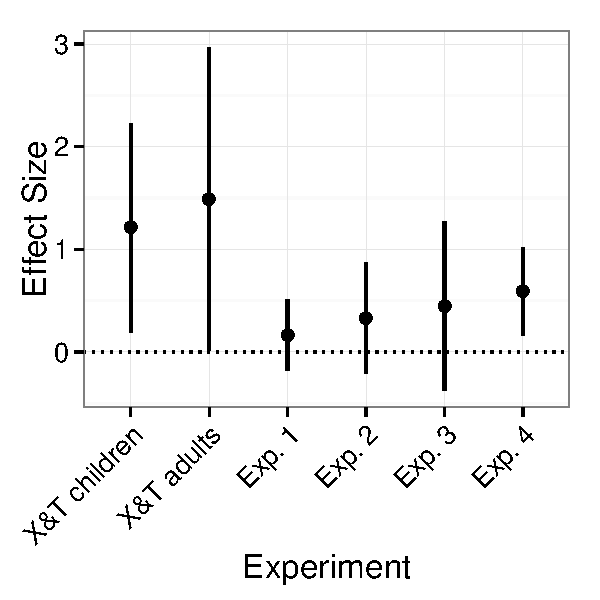
\includegraphics[width=3in]{figures/FIG_3.pdf} 
  \caption{\label{fig:effect_sizes} Effect size for the original experiment with adults, and our four replication attempts.  Effect sizes were calculated using the log odds ratio (S\'{a}nchez-Meca, Mar\'{i}n-Mart\'{i}nez, \& Chac\'{o}n-Moscoso, 2003). Those shown here reflect the liberal generalization criteria described in the Main Text. Errors bars are 95\% confidence intervals. } 
\end{figure}




\section{Experiment 2}

\subsection{Methods}

\subsubsection{Participants} 
\subsubsection{Stimuli}



\subsubsection{Procedure}

\subsection{Results and Discussion}

\subsection{Conclusion}



\section{Experiment 3}

\subsection{Methods}

\subsubsection{Participants} 
\subsubsection{Stimuli}


\subsubsection{Procedure}

\subsection{Results and Discussion}

\section{Experiment 4}
* notable flip

\subsection{Methods}

\subsubsection{Participants} 
\subsubsection{Stimuli}


\subsubsection{Procedure}

\subsection{Results and Discussion}

\subsection{General Discussion}
The most striking thing about this result is not the fact that we replicated it, but how much smaller the effect is than the original, and how sensitive it is to other factors

- would be nice to have paradigm where sampling didn't come from learner in learning context (other random way)
- vary variability parametrically
- things that might matter:
* variability visually
* spatial structure
* feature of the teacher (reliable?)
* cost of getting it wrong ("good enough processing" - in communiation vs. turk)

\nocite{sanchez2003effect}

\bibliographystyle{apacite2}
\bibliography{biblibrary}

\newpage
\theappendix 
\end{document}
